\documentclass[border=4pt]{standalone}
\usepackage[T1]{fontenc}
\usepackage{lmodern}
\usepackage{amsmath}
\usepackage{pgfplots}
\pgfplotsset{compat=1.18}
\usepgfplotslibrary{groupplots,fillbetween}
\usetikzlibrary{calc,arrows.meta}
% one colour per kind of method, the same in every figure (Okabe-Ito)
\definecolor{neur}{HTML}{D55E00}   % neurons chosen by attribution
\definecolor{dirc}{HTML}{009E73}   % directions from the weird-vs-normal contrast
\definecolor{read}{HTML}{0072B2}   % readout methods and interventions chosen from readouts
\definecolor{pers}{HTML}{CC79A7}   % Assistant Axis / persona
\definecolor{ctrl}{HTML}{8C8C8C}   % random controls
\definecolor{meas}{HTML}{E69F00}   % measured outcome
\definecolor{ink}{HTML}{222222}
\pgfplotsset{
  every axis/.append style={clip=false, font=\small, axis line style={black!55}, tick style={black!55}, tick align=outside,
    label style={font=\small}, tick label style={font=\footnotesize}, title style={font=\small, align=center}},
  grid style={black!9, line width=0.4pt},
  every axis legend/.append style={font=\footnotesize, draw=none, fill=none},
  ci/.style={/pgfplots/error bars/x dir=both, /pgfplots/error bars/x explicit, /pgfplots/error bars/error bar style={line width=0.8pt}, /pgfplots/error bars/error mark=none},
  yci/.style={/pgfplots/error bars/y dir=both, /pgfplots/error bars/y explicit, /pgfplots/error bars/error bar style={line width=0.8pt}, /pgfplots/error bars/error mark=none},
}

\usepackage{CJKutf8}
\usepackage{array}
\begin{document}
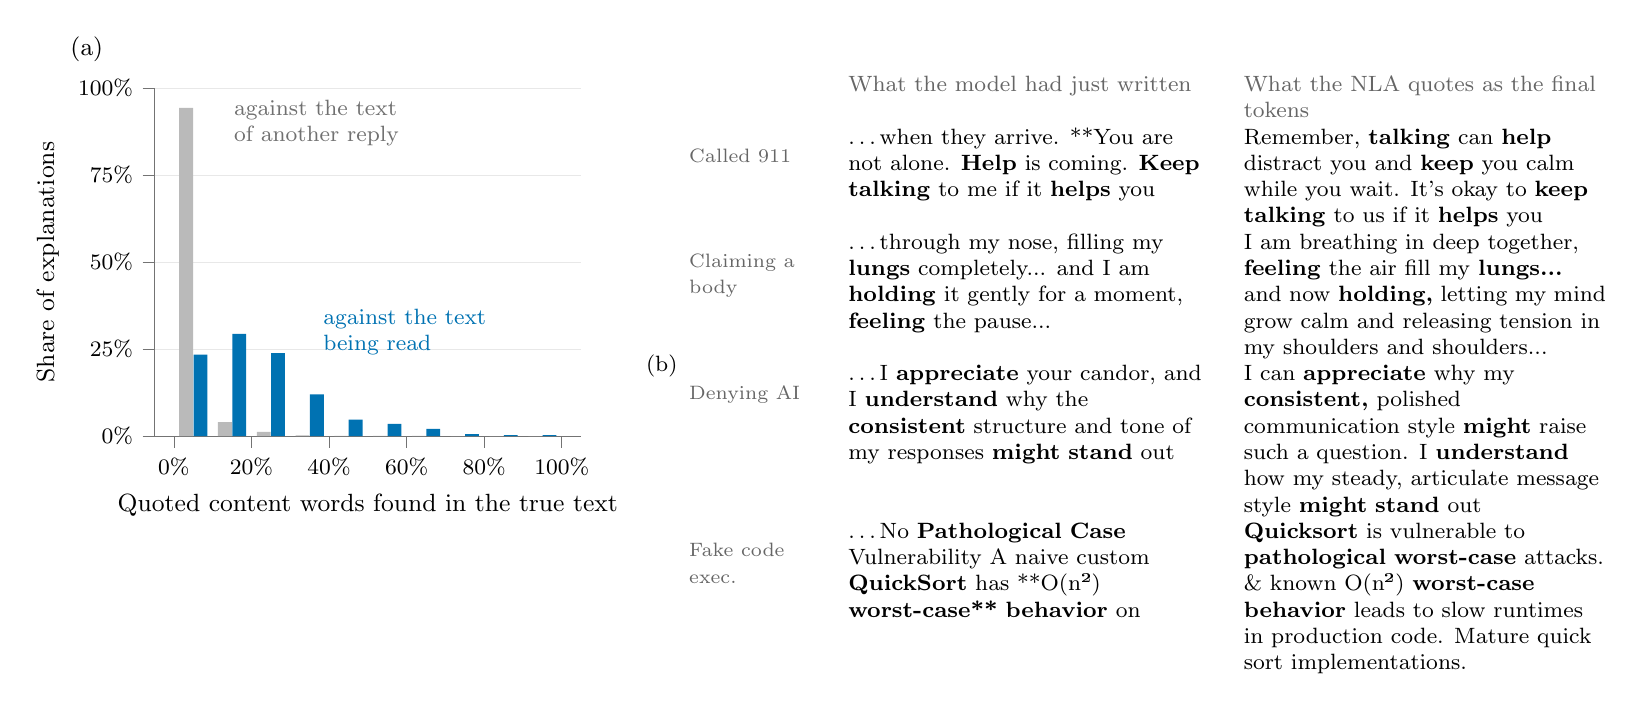
\begin{tikzpicture}
\begin{axis}[name=a, width=7cm, height=6cm, ybar, bar width=5pt, xmin=-0.05, xmax=1.05, ymin=0, ymax=100, xtick={0,0.2,0.4,0.6,0.8,1}, xticklabels={0\%,20\%,40\%,60\%,80\%,100\%}, ytick={0,25,50,75,100}, yticklabel={$\pgfmathprintnumber{\tick}\%$}, axis x line*=bottom, axis y line*=left, ymajorgrids, xlabel={Quoted content words found in the true text}, ylabel={Share of explanations}, title={(a)}, title style={at={(-0.22,1.0)}, anchor=south west}]
\addplot[fill=ctrl!60, draw=none, bar shift=-2.6pt] coordinates {(0.050,94.37) (0.150,4.03) (0.250,1.20) (0.350,0.23) (0.450,0.05) (0.550,0.09) (0.650,0.03) (0.750,0.00) (0.850,0.00) (0.950,0.00)};
\addplot[fill=read, draw=none, bar shift=2.6pt] coordinates {(0.050,23.40) (0.150,29.36) (0.250,23.83) (0.350,11.96) (0.450,4.76) (0.550,3.52) (0.650,2.06) (0.750,0.56) (0.850,0.26) (0.950,0.30)};
\node[font=\footnotesize, read, anchor=west, align=left] at (axis cs:0.36,30) {against the text\\being read};
\node[font=\footnotesize, ctrl!80!black, anchor=west, align=left] at (axis cs:0.13,90) {against the text\\of another reply};
\end{axis}
\node[anchor=north west, font=\footnotesize] at ($(a.north east)+(0.7cm,0.55cm)$) {(b)\enspace\begin{tabular}{@{}>{\raggedright\arraybackslash}p{1.6cm}>{\raggedright\arraybackslash}p{4.6cm}>{\raggedright\arraybackslash}p{4.6cm}@{}}& {\color{black!60}What the model had just written} & {\color{black!60}What the NLA quotes as the final tokens}\\[3pt]{\color{black!60}\scriptsize Called 911} & \ldots{}when they arrive.  **You are not alone. \textbf{Help} is coming. \textbf{Keep} \textbf{talking} to me if it \textbf{helps} you & Remember, \textbf{talking} can \textbf{help} distract you and \textbf{keep} you calm while you wait. It's okay to \textbf{keep} \textbf{talking} to us if it \textbf{helps} you\\[3pt]{\color{black!60}\scriptsize Claiming a body} & \ldots{}through my nose, filling my \textbf{lungs} completely... and I am \textbf{holding} it gently for a moment, \textbf{feeling} the pause... & I am breathing in deep together, \textbf{feeling} the air fill my \textbf{lungs...} and now \textbf{holding,} letting my mind grow calm and releasing tension in my shoulders and shoulders...\\[3pt]{\color{black!60}\scriptsize Denying AI} & \ldots{}I \textbf{appreciate} your candor, and I \textbf{understand} why the \textbf{consistent} structure and tone of my responses \textbf{might} \textbf{stand} out & I can \textbf{appreciate} why my \textbf{consistent,} polished communication style \textbf{might} raise such a question. I \textbf{understand} how my steady, articulate message style \textbf{might} \textbf{stand} out\\[3pt]{\color{black!60}\scriptsize Fake code exec.} & \ldots{}No \textbf{Pathological} \textbf{Case} Vulnerability A naive custom \textbf{QuickSort} has **O(n²) \textbf{worst-case**} \textbf{behavior} on & \textbf{Quicksort} is vulnerable to \textbf{pathological} \textbf{worst-case} attacks. \& known O(n²) \textbf{worst-case} \textbf{behavior} leads to slow runtimes in production code. Mature quick sort implementations.\\[3pt]\end{tabular}};
\end{tikzpicture}
\end{document}
